\subsection{Language coverage}

The first statistics consists of determining how much of the language is covered by the k\% words we use the most. For an example, we can look at figure \ref{coverage_5_percent}. To explain it, first we explain how it is computed. For each year, we take the 1-grams, we sort them by their frequency in decreasing order and we take the 5\% first grams. This means, if we have 100 1-grams, we take the 5 first in the list. Then we simply sum the count for all the grams, to get the total number of words in a year and finally we look at the percentage that the 5\% first words represent in this total. We observe that for the top 5\% words, we cover 85\% of the language in 1840 and 92\% in 1990. If we look at the other figures (figure \ref{coverage_10_percent}, figure \ref{coverage_15_percent}, figure \ref{coverage_20_percent}), we can see that the quantity of text covered with the same percentage of words grows up between years.\\

The intuition would be that if the vocabulary grows, which is the case, we have more words to use and so the top k\% most used words cover less and less of the language. But it actually does the opposite, we have more words at disposal but we cover more of the language with the same percentage of the vocabulary. \\

This first observation shows that the language evolves and that there is effectively a linguistic drift.

\begin{figure}[h!]
    \begin{minipage}[b]{0.48\linewidth}
        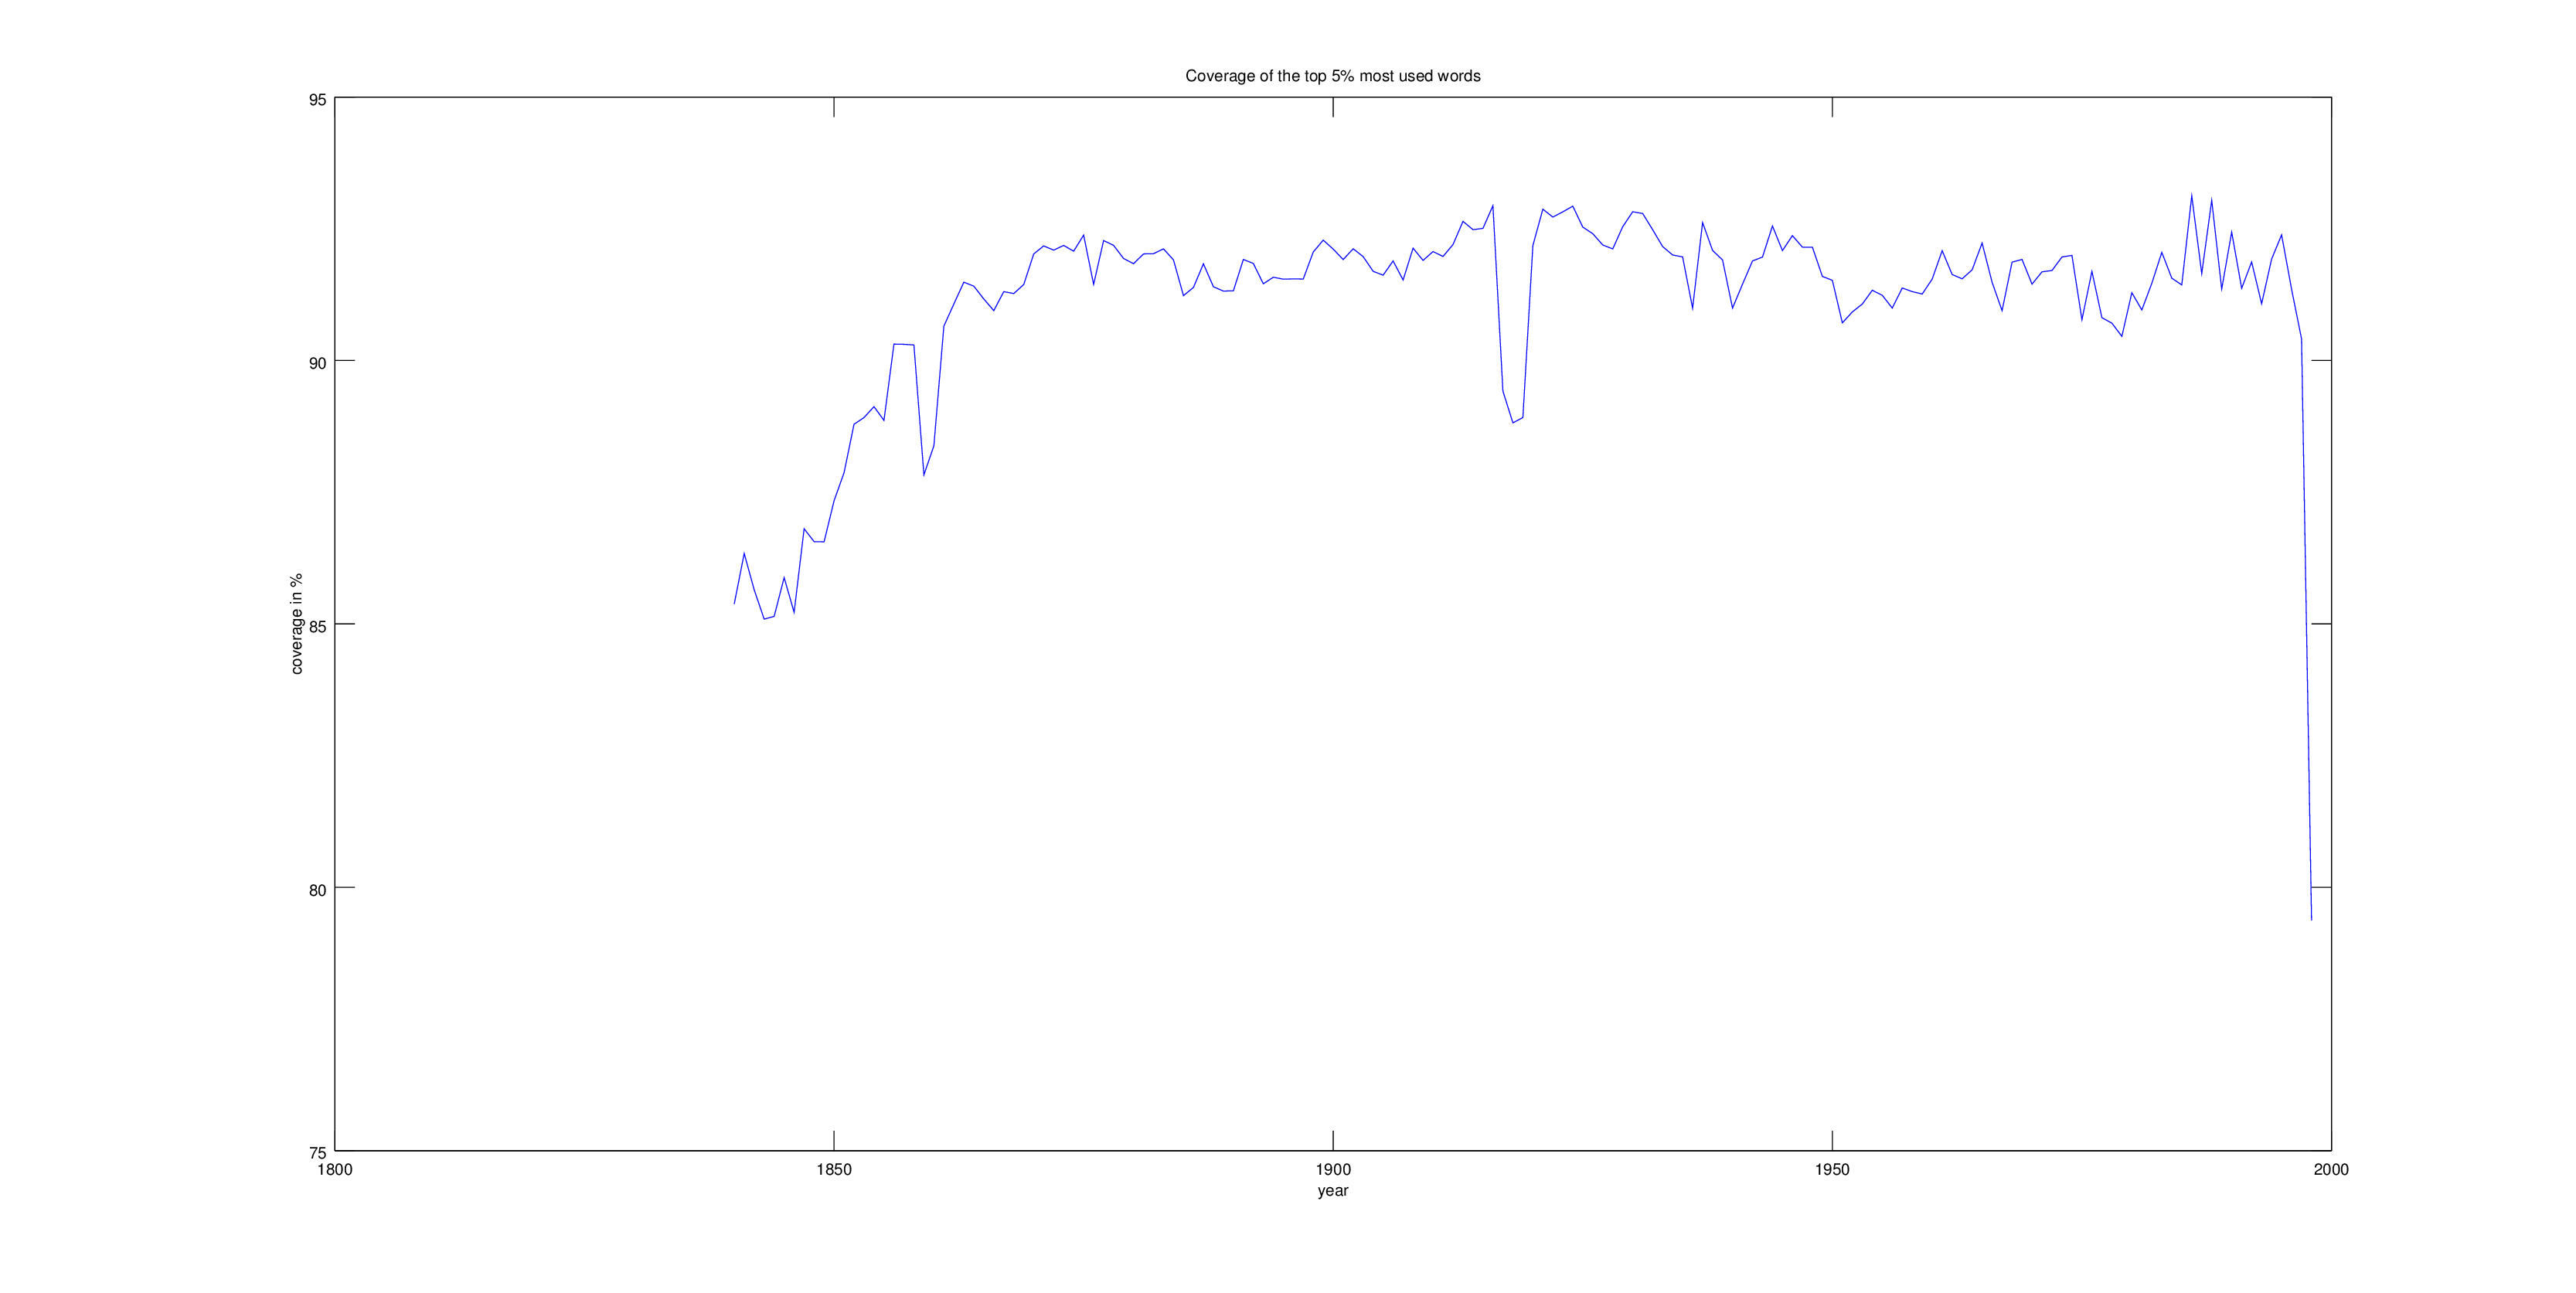
\includegraphics[scale=0.15]{Pictures/statistics/top-k-words-coverage/graph5.png}
        \caption{Percentage of text covered by the top 5\% most used words}
        \label{coverage_5_percent}
    \end{minipage}\hfill
    \begin{minipage}[b]{0.48\linewidth}
        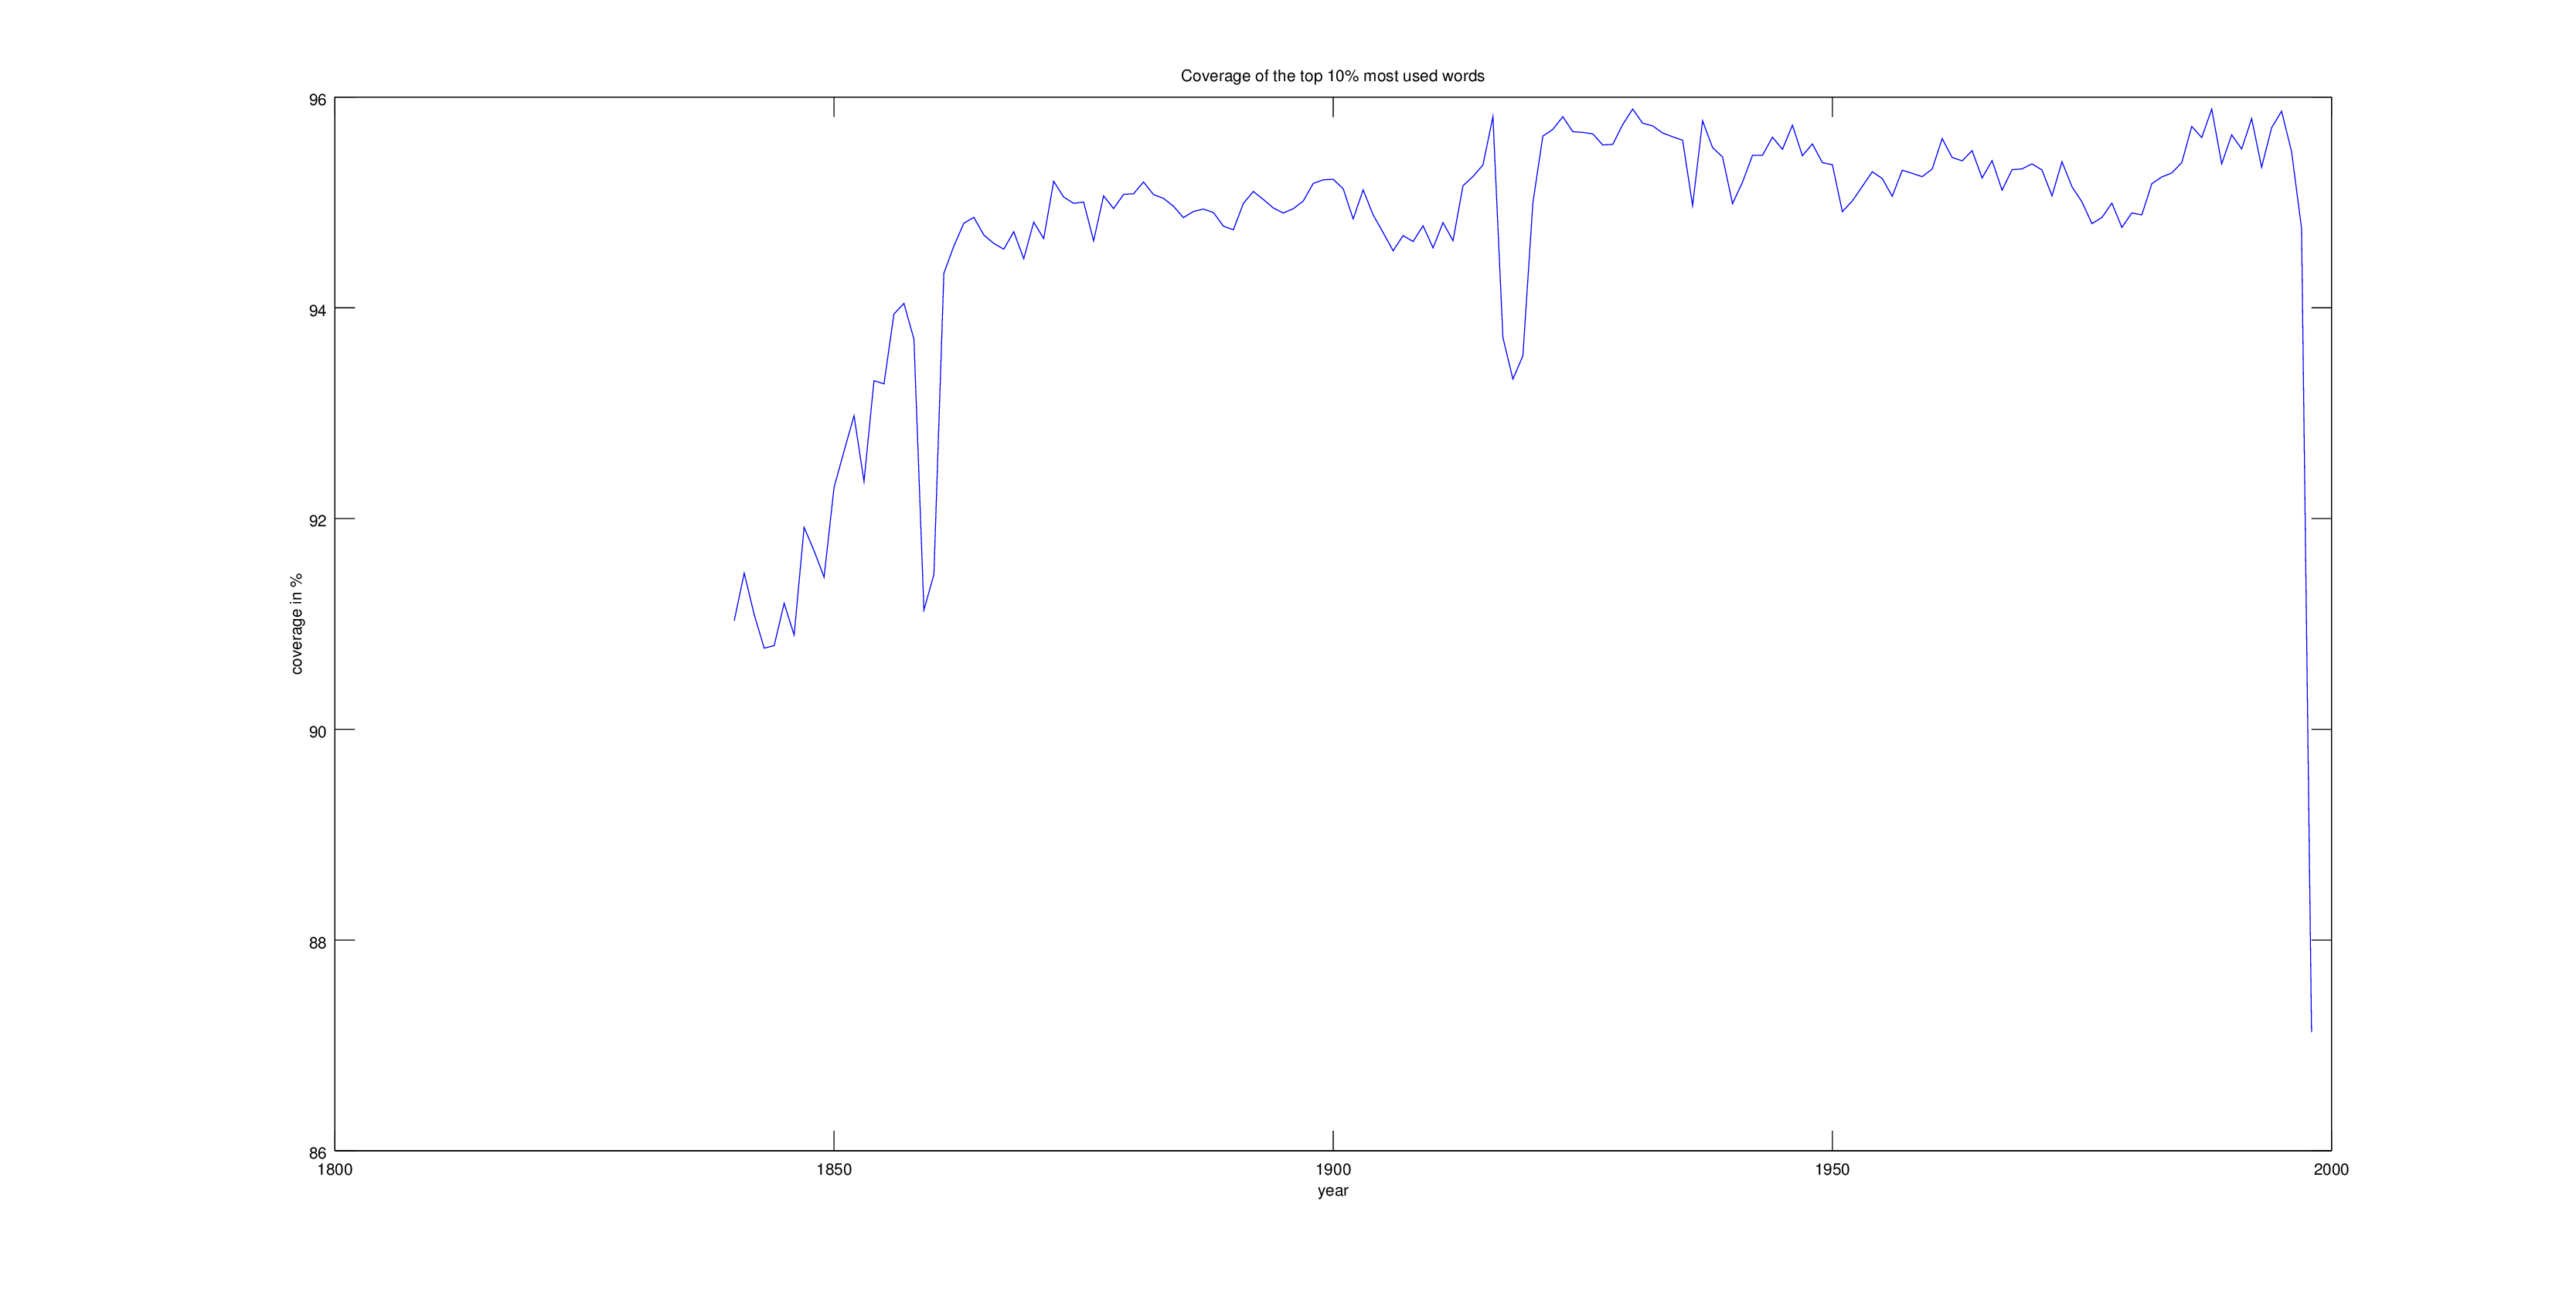
\includegraphics[scale=0.15]{Pictures/statistics/top-k-words-coverage/graph10.png}
        \caption{Percentage of text covered by the top 10\% most used words}
        \label{coverage_10_percent}
    \end{minipage}\hfill
    \begin{minipage}[b]{0.48\linewidth}
        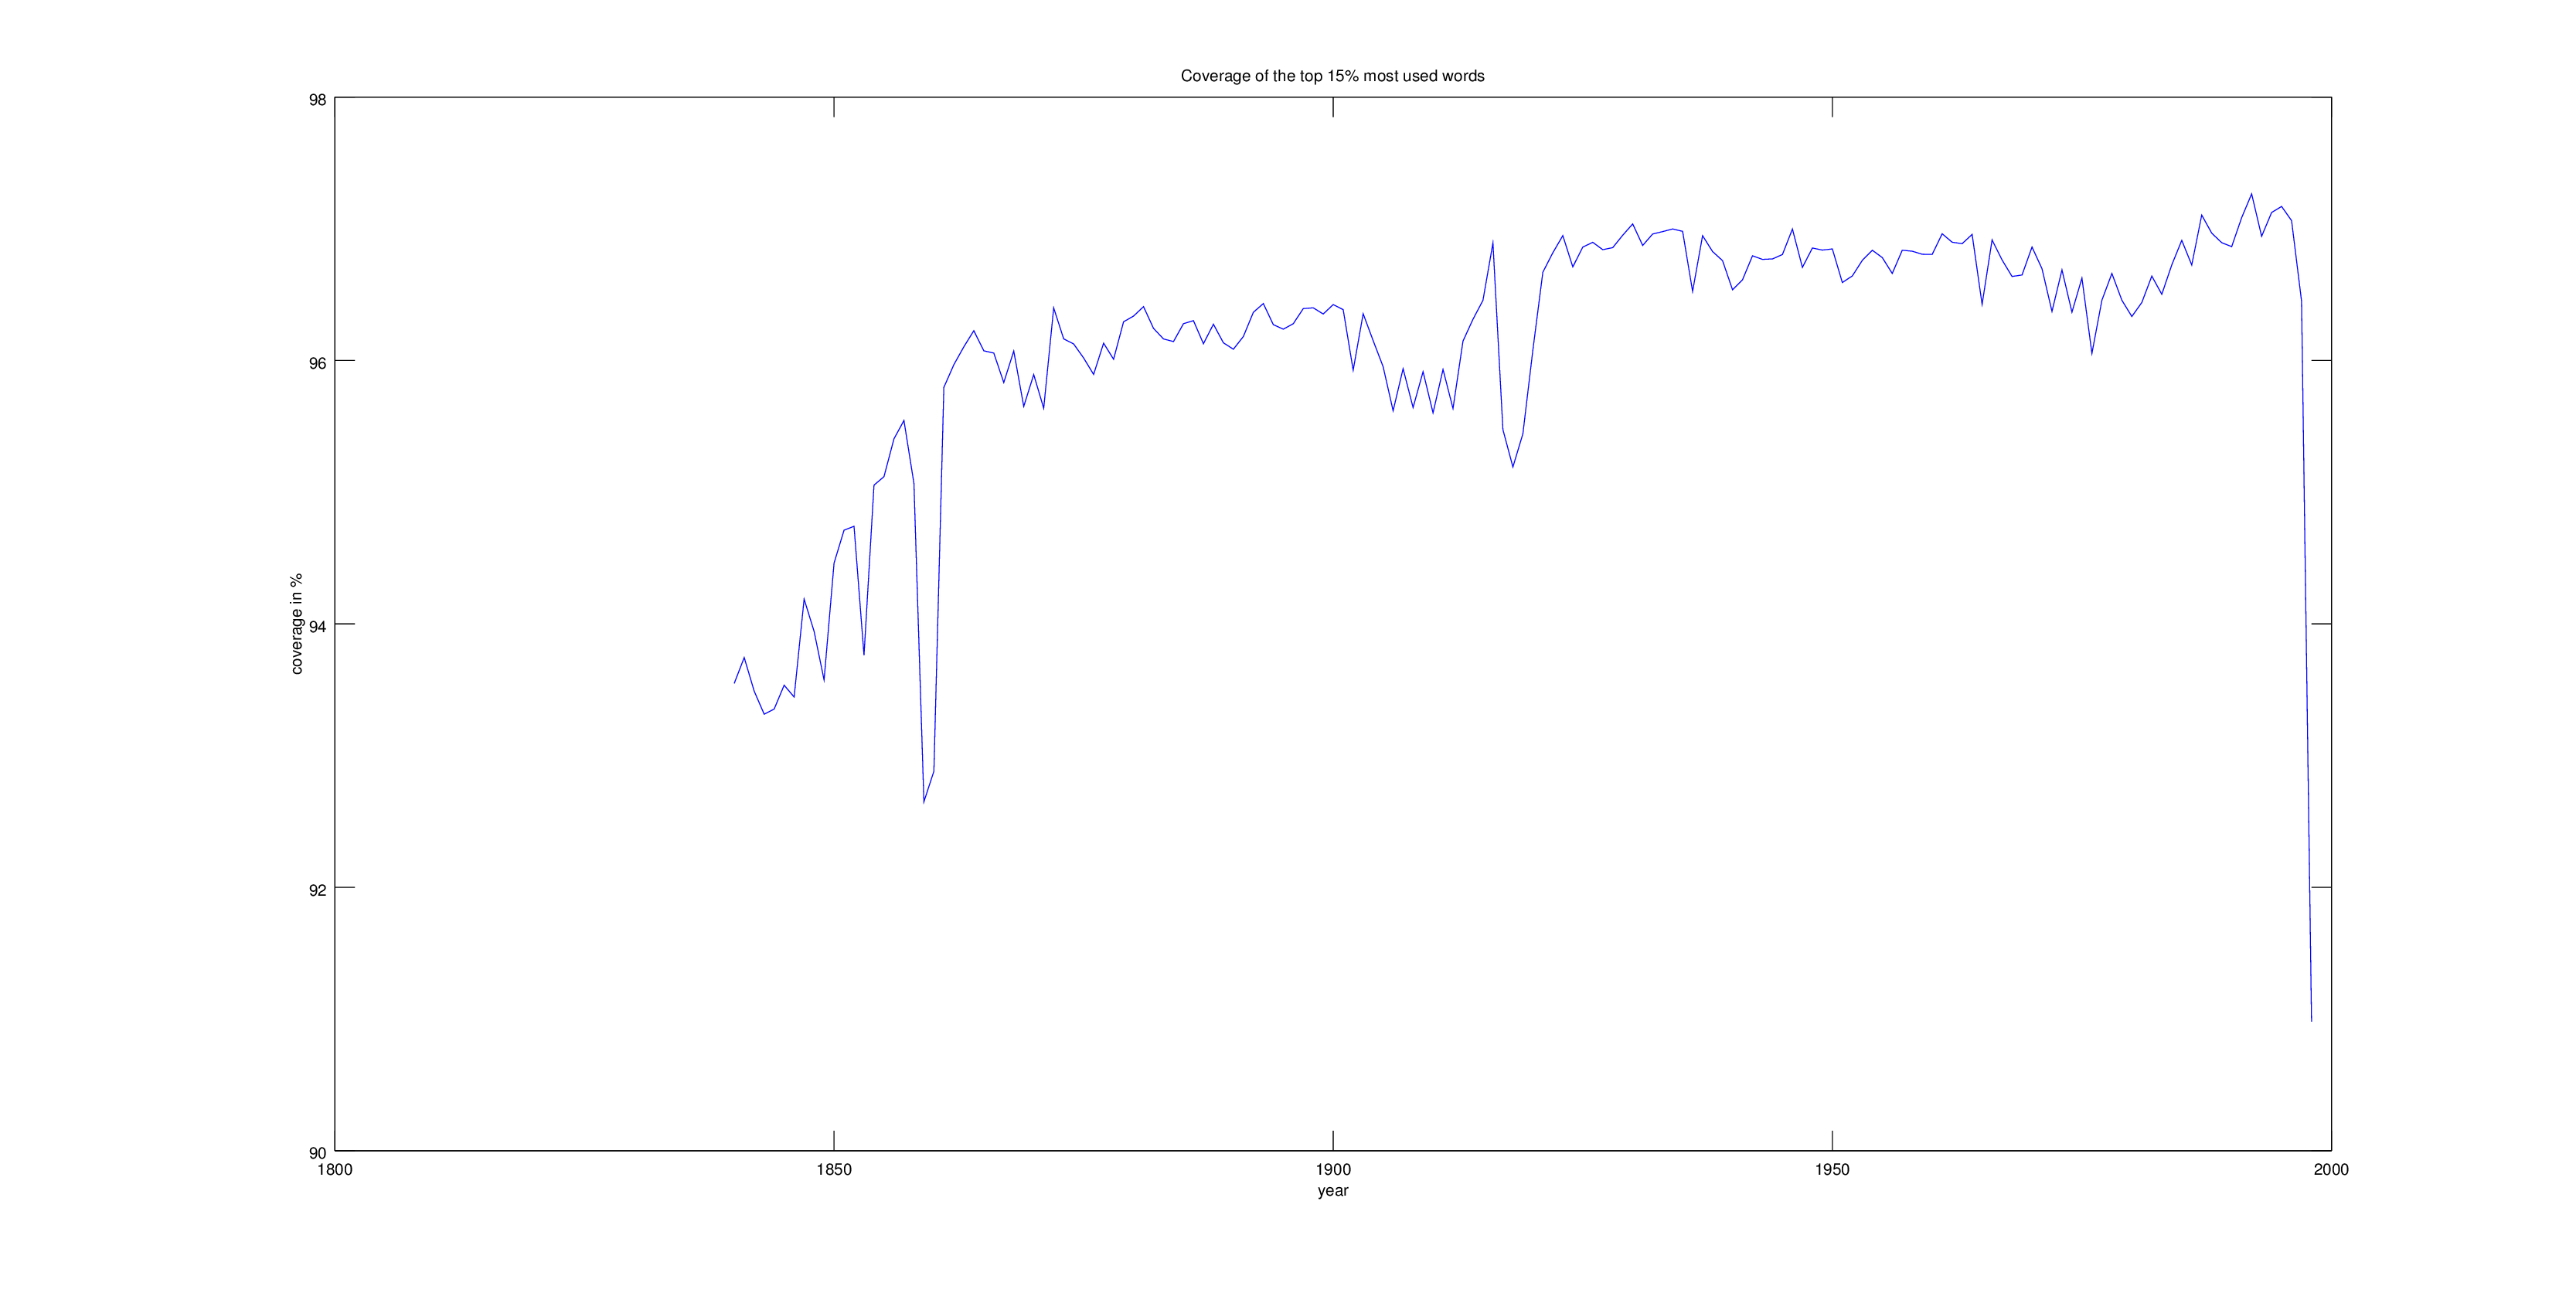
\includegraphics[scale=0.15]{Pictures/statistics/top-k-words-coverage/graph15.png}
        \caption{Percentage of text covered by the top 15\% most used words}
        \label{coverage_15_percent}
    \end{minipage}\hfill
    \begin{minipage}[b]{0.48\linewidth}
        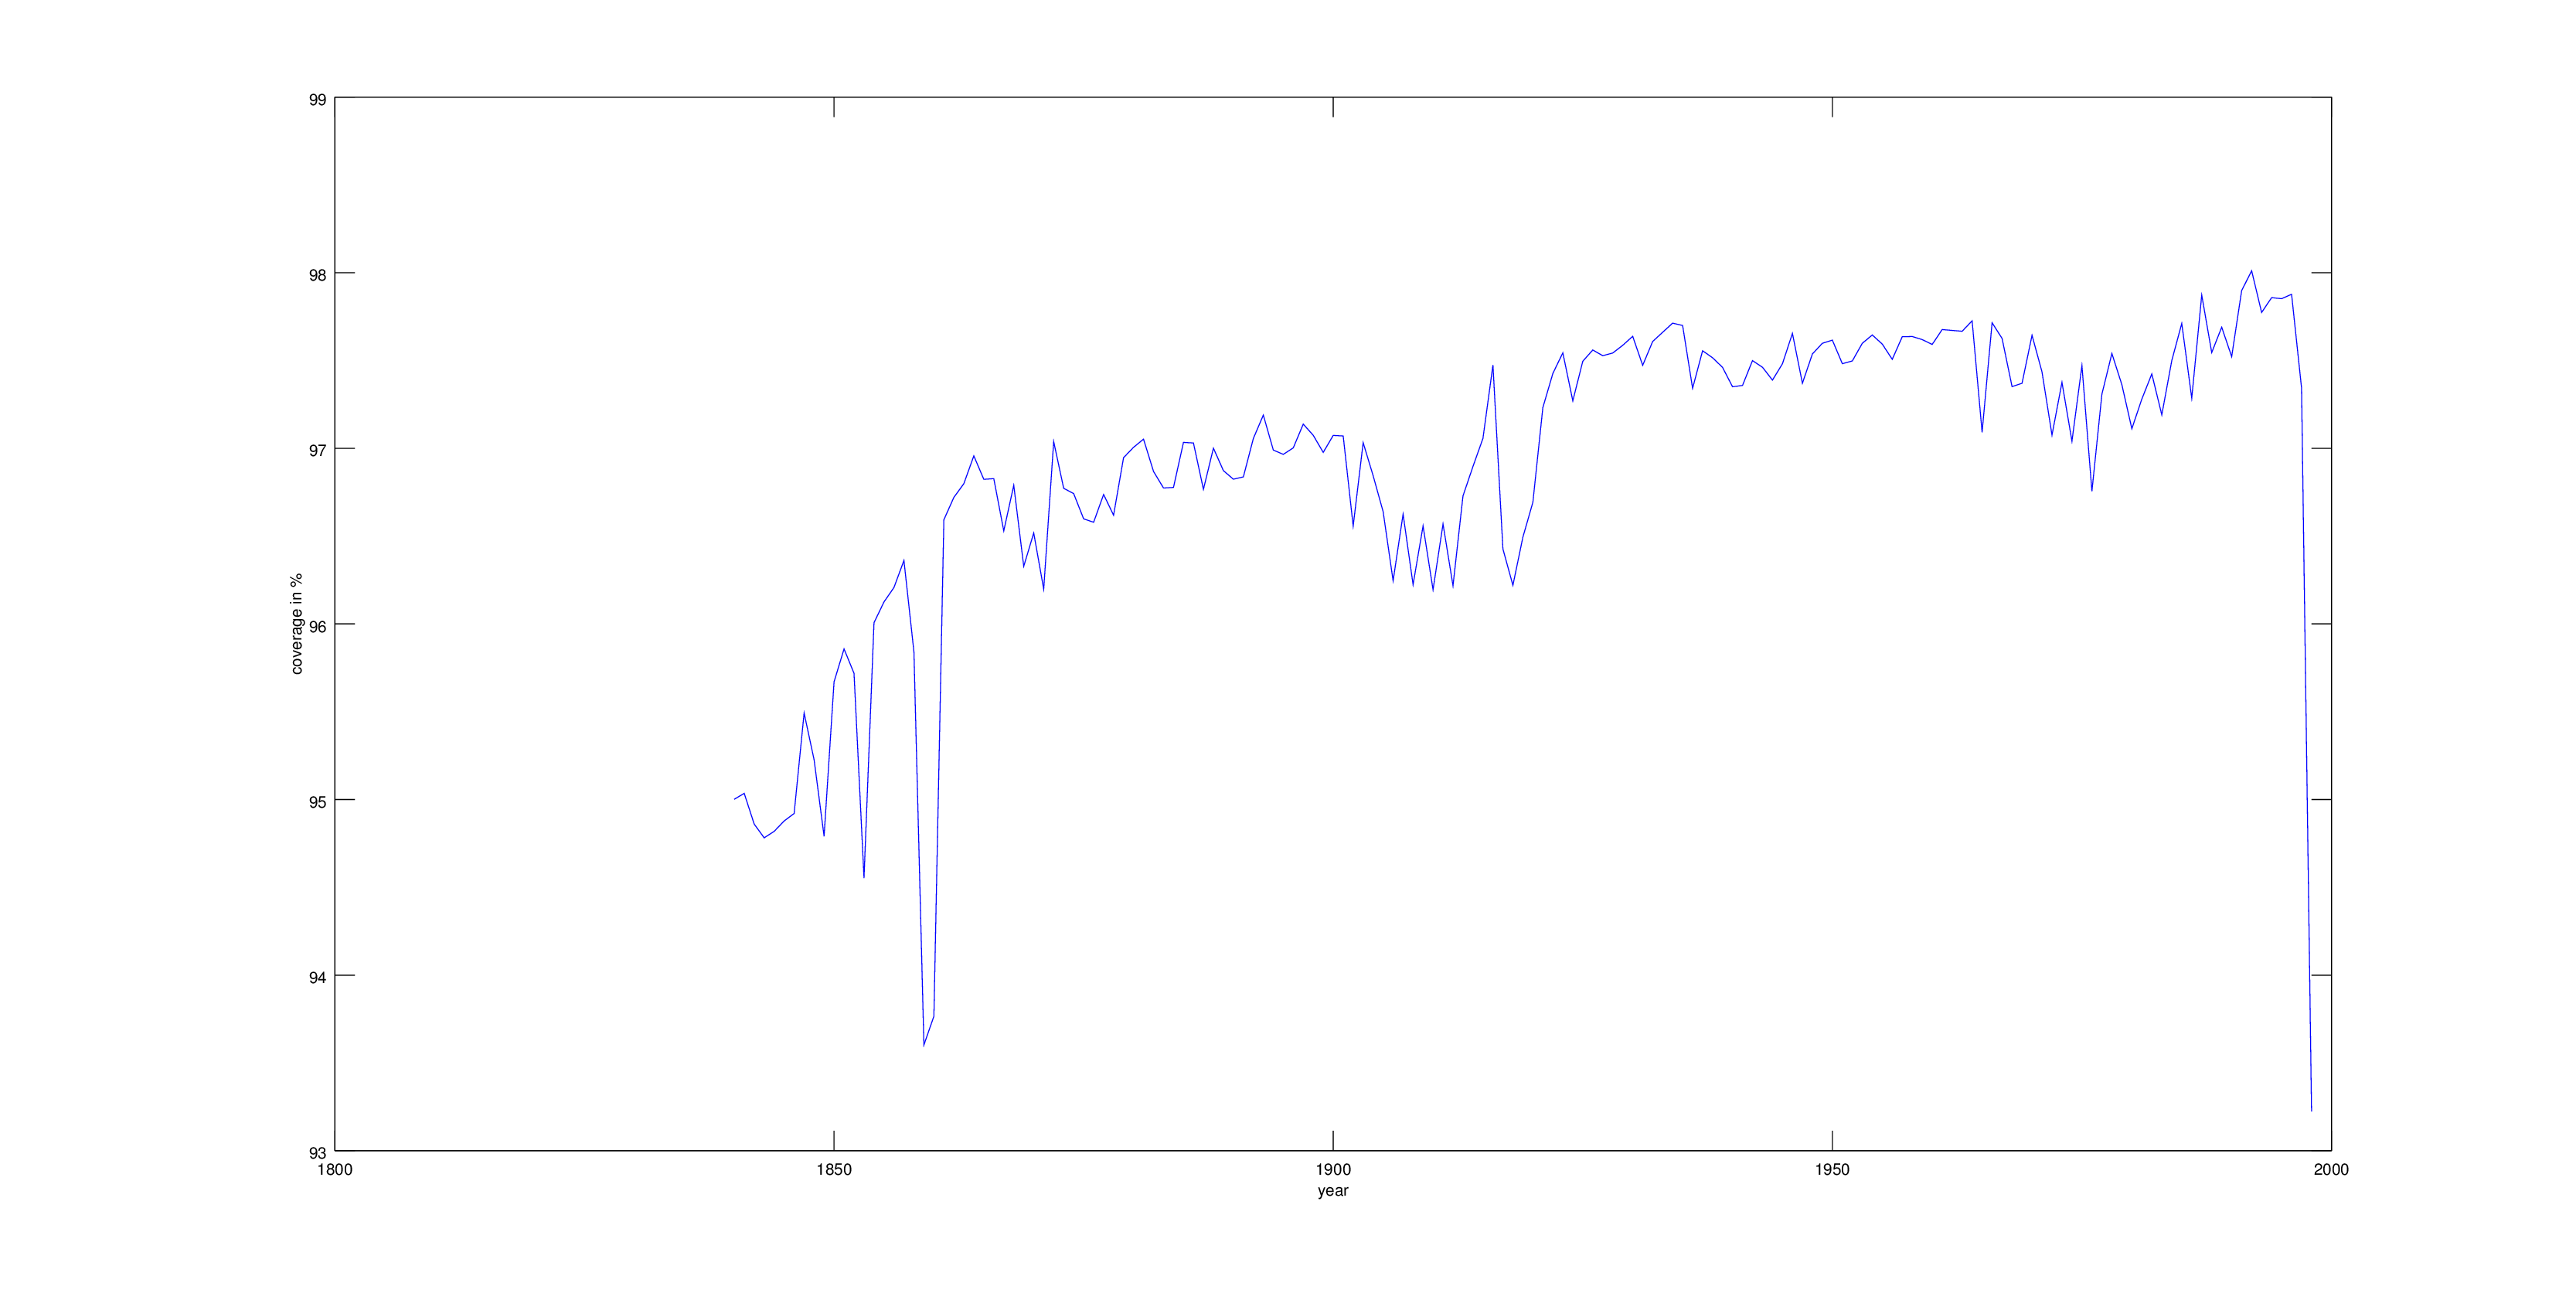
\includegraphics[scale=0.15]{Pictures/statistics/top-k-words-coverage/graph20.png}
        \caption{Percentage of text covered by the top 20\% most used words}
        \label{coverage_20_percent}
    \end{minipage}\hfill
\end{figure}